\subsection{SPPF analysis and semantics calculation}

The result of dynamically generated expressions parsing is a parse forest represented by the structure called SPPF~\cite{SPPF:ref}. This structure allows to reuse common subtrees for different trees.

Based on SPPF it is possible to build a so called compound control flow graph and try to solve classic static analysis tasks using it. When building compound CFG we assume that the string-embedded language grammar is a grammar of some programming language and that a mapping between non-terminals and CFG blocks is defined. For instance the \verb|"if_stmt"| non-terminal derivation should be treated as the conditional block in CFG. Other example is shown in Figure~\ref{simple_example_pic}, where the \verb|"assignment"| non-terminal derivation is treated as the assignment operation in CFG.

\begin{figure}[h!]
  \begin{center}
    \begin{subfigure}{0.3\textwidth}    
        \includegraphics[scale=0.3]{Graphs/cfg_idea.eps}    
    \caption{}
    \label{simple_a}
    \end{subfigure}
    \begin{subfigure}{0.1\textwidth}      
            \includegraphics[scale=0.5]{Graphs/assignment_simple.eps}        
     \caption{}
     \label{simple_b}
    \end{subfigure}
    \caption{\texttt{assignment} non-terminal derivation (\ref{simple_a}) and corresponding CFG block (\ref{simple_b})}
    \label{simple_example_pic}
  \end{center}
\end{figure}

Because of the fact that SPPF can contain several trees, the compound CFG can contain several usual CFGs. To make this possible an intermediate nodes are introduced. Further intermediate nodes will be called \textit{"nodes"} (in figures they will have oval shape) and CFG elements will be called \textit{"blocks"} (in the figures they will have rectangle shape). The derivation of \verb|"assignment"| non-terminal corresponding to sequences \verb|"X = 1;"| and \verb|"Y = 1;"| is shown in Figure~\ref{complicated_example_pic}. 

\begin{figure}[h!]
    \begin{center}
    \begin{subfigure}{0.3\textwidth}    
        \includegraphics[scale=0.3]{Graphs/cfg_idea_complicated.eps}    
    \caption{}
    \label{complicated_a}
    \end{subfigure}
    \begin{subfigure}{0.1\textwidth}      
            \includegraphics[scale=0.5]{Graphs/assignment_complicated.eps}
        \caption{}
        \label{complicated_b}
    \end{subfigure}
    \caption{\texttt{"assignment"} non-terminal derivation (\ref{complicated_a}) and corresponding CFG blocks (\ref{complicated_b})}
    \label{complicated_example_pic}
    \end{center}
\end{figure}
Using obtained compound CFG one can solve the static analysis tasks. Consider definite assignment analysis as an example. Here we suppose that variable is defined in the statement $\alpha$ if and only if there is a variable definition along each of the evaluation paths from the program's start to the $\alpha$ statement. 

For each block $\alpha$ the following transitions are valid:
$$
before (\alpha) \;=\; \bigcap_{\beta \;\in\; pred(\alpha)} \;after(\beta)
$$
$$
after (\alpha) \;=\; before(\alpha) \cup gen(\alpha)
$$
where
\begin{itemize}
\item $before(\alpha)$ set contains variables defined before the statement $\alpha$;
\item $after(\alpha)$ set contains variables defined after the statement $\alpha$;
\item $gen(\alpha)$ set is empty if $\alpha$ is not an assignment block and contains left-hand operand of the assignment otherwise. 
\end{itemize}

As in case of usual CFG, the algorithm traverses the graph beginning from the start node for which the empty set is associated with. The only difference is that the $pred(\alpha)$ set contains nodes, not CFG blocks. But it is easy to define the required sets:
$$
before (\beta) \;=\; \bigcap_{\alpha \;\in\; pred(\beta)} \;after(\alpha)
$$
$$
after (\beta) \;=\; before (\beta)
$$
The compound CFG is shown in Figure~\ref{cfg_example}. In the red colored node only variable \verb|X| is defined. This node have two child blocks and the list containing variable \verb|X| is passed to each block. The \verb|"Y = X + 2;"| block adds the variable \verb|Y| to the list (because \verb|Y| is defined in this block), and the \verb|"Z = X * 3;"| block adds the variable \verb|Z|. These two blocks have the same child node, therefore the intersection of parents' lists is associated with it, i.e. the list containing the only variable \verb|X|. The list is passed when the block \verb|"X = Y * Z;"| is processed. Since passed list does not contain \verb|Y| and \verb|Z|, they will be reported as undefined variables.
\begin{figure}[h!]
    \begin{center}
        \includegraphics[scale=0.4]{Graphs/cfg_example.eps}
    \end{center}
    \caption{Compound control flow graph}
    \label{cfg_example}
\end{figure} 
